\documentclass[dvipdfmx, tikz]{standalone}
\usepackage{tikz}
\usetikzlibrary{calc,decorations.pathreplacing,quotes,positioning,shapes,fit,arrows,backgrounds,tikzmark}

\begin{document}
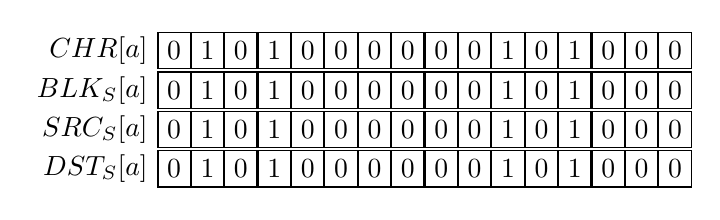
\begin{tikzpicture}[state/.style={circle, draw, minimum size=.7cm}, node distance=0cm]
  \node(chr0) [rectangle, draw] at (0,0) {$0$};
  \node(chr) [left =of chr0] {$CHR[a]$};
  \foreach \x [count=\i from 0, remember=\i as \prev (initially 0)] in {1,0,1,0,0,0,0,0,0,1,0,1,0,0,0} {
		\node(chr\i) [rectangle, draw, right =of chr\prev] {$\x$};
	}

  \node(blk0) [rectangle, draw] at (0,-.5) {$0$};
  \node(blk) [left =of blk0] {$BLK_S[a]$};
  \foreach \x [count=\i from 0, remember=\i as \prev (initially 0)] in {1,0,1,0,0,0,0,0,0,1,0,1,0,0,0} {
		\node(blk\i) [rectangle, draw, right =of blk\prev] {$\x$};
	}

  \node(src0) [rectangle, draw] at (0,-1) {$0$};
  \node(src) [left =of src0] {$SRC_S[a]$};
  \foreach \x [count=\i from 0, remember=\i as \prev (initially 0)] in {1,0,1,0,0,0,0,0,0,1,0,1,0,0,0} {
		\node(src\i) [rectangle, draw, right =of src\prev] {$\x$};
	}

  \node(dst0) [rectangle, draw] at (0,-1.5) {$0$};
  \node(dst) [left =of dst0] {$DST_S[a]$};
  \foreach \x [count=\i from 0, remember=\i as \prev (initially 0)] in {1,0,1,0,0,0,0,0,0,1,0,1,0,0,0} {
		\node(dst\i) [rectangle, draw, right =of dst\prev] {$\x$};
	}
\end{tikzpicture}
\end{document}
